\chapter[Transiting Exoplanets]%
{%
Transiting Exoplanets}
\label{cha:intro}

\section{The Search for Other Worlds Using Starlight}
\label{cha:intro:sec:search}

Astronomy in the 21st century has seen significant progress made in the age-old question of our uniqueness in the universe.
Less than two decades since the first discoveries of planetary-mass systems around stars other than our Sun \citep{Latham_Stefanik_Mazeh:nat:1989a, Wolszczan_Frail:nat:1992a, Mayor_Queloz:nat:1995a}, we now know of 200 planetary systems, and the rate of new discoveries is increasing.
The planets in these new systems are known as ``extrasolar planets'' or ``exoplanets'' for short.

Since the reflected or emitted light from a planet is very dim compared with starlight, the vast majority of detections have been made by studying the light from the host star as the star interacts with the planet.
Software and hardware improvements have made possible the detection of minute changes in observations of these stars.
This thesis work, and the study of exoplanets in general, utilizes telescopes both on the ground and in space, and ranging from ten-centimeter to ten-meter in diameter.
With these tools, we are able to test our understanding of how gas giants are formed and how their internal structure and chemical composition vary with environment.
With each new discovery, we make another step toward the detection of a solar system analog or a mirror Earth in the habitable zone of a star.

Before continuing, it should be noted that a distinction is made---by the International Astronomical Union (IAU), if not by nature---between different types of stellar companions that are thereby segregated by mass.
The evolution of celestial objects that fuse \textit{hydrogen} in their cores is quite different from the evolution of objects without this fusion.
Hence, only the \textit{hydrogen}-burning bodies (those that have at least 80 times the mass, \mjup, of Jupiter) are called \textit{stars}.
Objects that are less massive than stars, yet can fuse \textit{deuterium} in their cores, are known as {\it brown dwarfs}, and have masses greater than 13\,\mjup.
Finally, the least massive stellar companions are {\it planets}.
The latter are the target of my survey, and the planets found during this thesis work have masses $\mp\sim\mjup$, well below the 13\,\mjup\ limit, hence different interpretations of the mass boundaries will not affect my results.

\section{Methods for Detecting Hot Jupiters and Other Exoplanets}
\label{cha:intro:sec:methods}

The majority of the known exoplanetary systems contain planets similar in mass to Jupiter and the other solar system giant planets, rather than the lighter terrestrial planets such as Earth.
This is because most of the exoplanets were found by measuring a change in the motion of their star caused by the gravitational presence of the orbiting planet, a method that is inherently more sensitive to massive planets.
The velocity of a star in space can be split into two components: the {\it radial velocity} along the line of sight to the star (either toward or away from us), and the {\it tangential velocity} across the sky, perpendicular to the line of sight.
Although there are several other successful methods to find exoplanets, in this thesis I will concentrate on a planet search that uses the measurement of radial-velocity variations to confirm the existence of planets observed to transit across stellar disks.

\subsection{Radial Velocities}
\label{cha:intro:sec:methods:sub:rv}

The radial velocity of a star is determined from the Doppler shifts of the stellar spectral lines due to the motion of the star.
By measuring the variation with time of the radial velocities of the star (of mass \mstar) and deriving the stellar orbit around the barycenter of the system, we can determine several orbital parameters of the planet, such as the orbital period $P$
and the eccentricity $e$.
We can also estimate its mass, or at least a lower limit to the mass, from these orbital parameters and the amplitude of the variation.
The product of the planetary mass $\mp$ and the sine of the orbital inclination $i$ can be computed from the mass function:
\begin{eqnarray*}
\frac{(\mp \sin{i})^3}{(\mstar + \mp)^2} & =
& \frac{P K^3}{2 \pi G}  (1-e^2)^{3/2},
\end{eqnarray*}
where $K$ is the {\it semi}-amplitude of the radial velocity variation and $G$ is the universal gravitational constant.
This product is known as the minimum mass of the planet.
Assuming a circular orbit and that $\mp << \mstar$, we can write this as:
\begin{eqnarray}
\mp \sin{i} & \simeq & 1\,\mjup \left( \frac{K}{200\,\ms} \right)
    \left( \frac{P}{\mathrm{day}} \right)^{1/3}
    \left( \frac{\mstar}{\msun} \right)^{2/3}.\label{cha:intro:sec:methods:sub:rv:eqn:mpsini}
\end{eqnarray}
Thus, the gravitational effect of Jupiter on the Sun is quite small, resulting in a motion of     12.5\,\ms\ or 45\,$\mathrm{km\,hr^{-1}}$, whereas a 1\,\mjup\ planet in a one-day period around the sun would induce a motion of $K=200\,\ms$.
The ability to measure from many parsecs away these small orbital accelerations requires measuring shifts in the stellar spectral lines with a precision of roughly one thousandth of the width of a spectral line.
Hardware and software developments have improved this precision to the point where it is possible to detect planets with minimum masses of $\sim$5\,\mearth ($\sim$0.02\,\mjup; e.g., \mbox{Gliese 581c}; \citealp{Udry_Bonfils_Delfosse:aa:2007a}).

Although the radial-velocity surveys are the most prolific planet campaigns, they suffer from several limitations.
The target stars are observed one at a time, requiring a heavy investment of large telescope time.
The surveys are restricted to the brightest stars in the sky, again due to limited telescope resources.
Finally, the precision of these measurements is not likely to be indefinitely improved, due to an astrophysical limit.
Stars are asteroseismically active, producing radial-velocity ``jitter'' on the scale of ~1--10\,\ms\ (\citealp*{Saar_Butler_Marcy:apjl:1998a}; \citealp{Santos_Mayor_Naef:aa:2000a, Wright:pasp:2005a}).
It is thought that this jitter will hinder achieving precisions much better than currently obtained.

\begin{figure}
\begin{center}
\centering
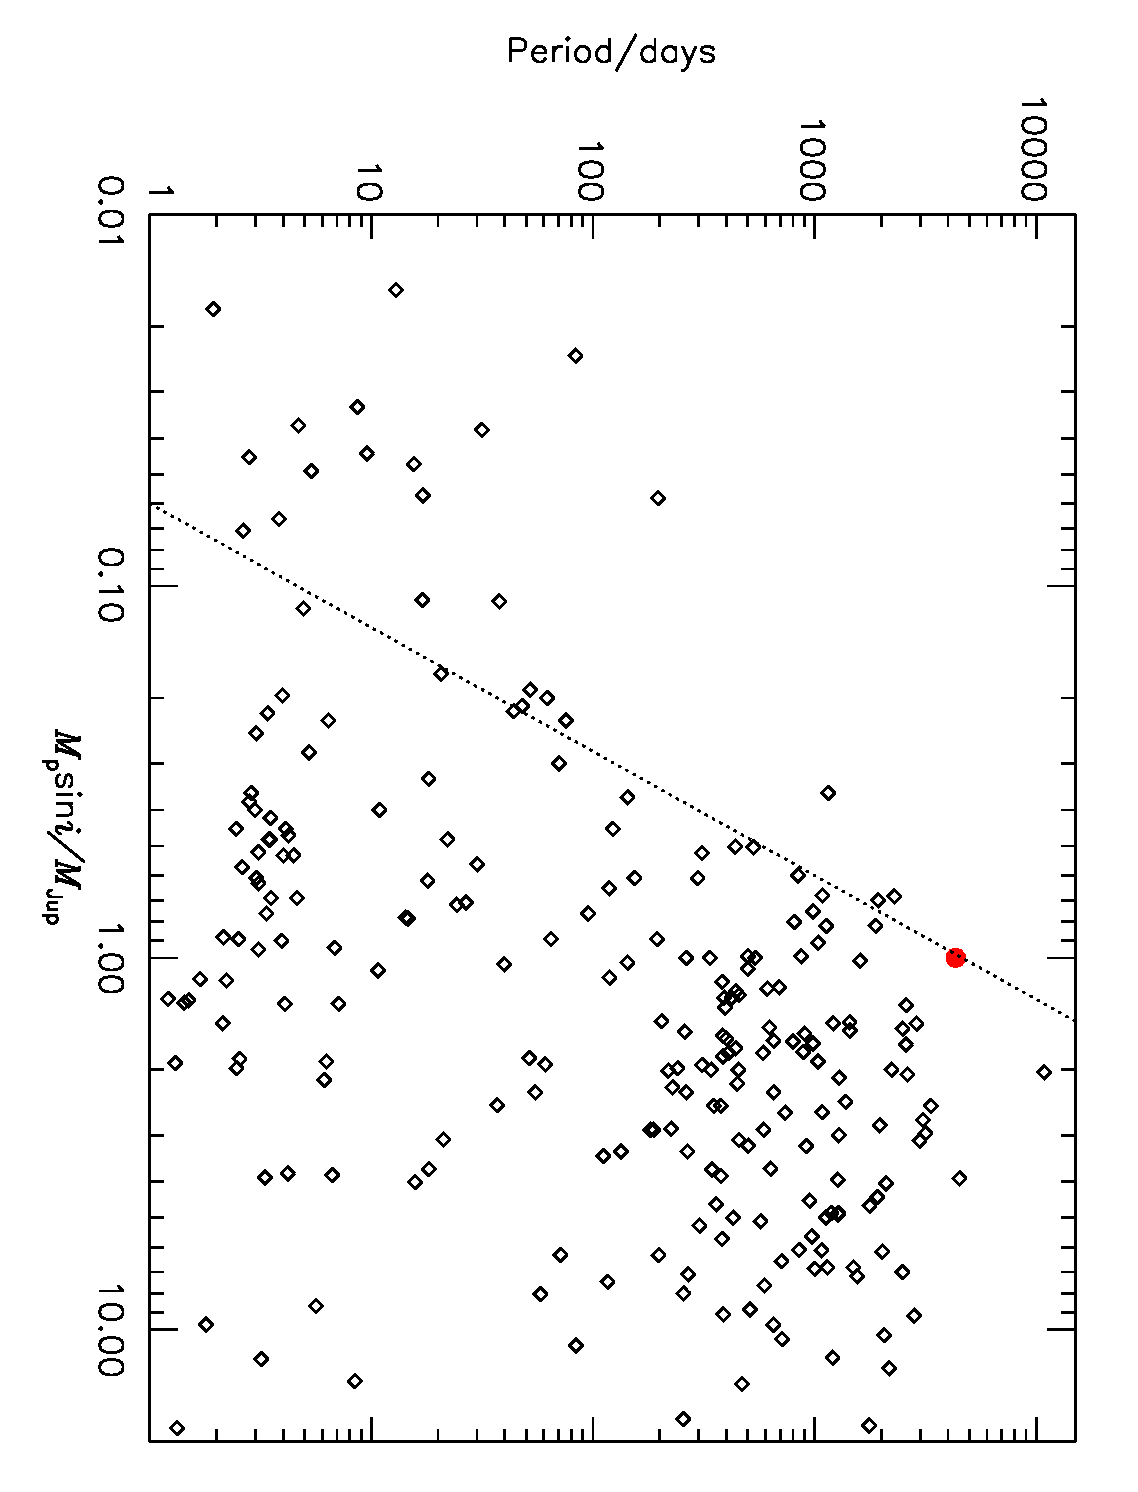
\includegraphics[angle=90,width=.90\textwidth]{1_rvplanets}
\caption[Orbital period distribution of the 232 known exoplanets]{%
Orbital period distribution of the 232 known exoplanets as a function of their minimum masses.
Jupiter is shown for comparison as a {\it red, filled circle}.
Relatively few massive planets with short orbital periods have been found, despite the bias for such planets in the radial-velocity surveys.
An approximate detection threshold (defined as $K=4\sigma$, see text) is shown as a {\it dotted line}.%
}
\label{cha:intro:sec:methods:sub:rv:fig:rv}
\end{center}
\end{figure}

The enlarging catalog of planets from radial-velocity surveys of stars in the solar neighborhood facilitates studying the statistics of exoplanets.
For example, the frequency of planets can be estimated from the yield of these surveys, and is currently estimated at $\sim$5\% for planets of 0.5--8\,\mjup\ within 3\,AU \citep{Udry_Fischer_Queloz:PPV2007a}.
There is a correlation between the metallicity of stars and this frequency of planets around them (\citealp{Gonzalez:mnras:1997a, Fischer_Valenti:asp:2003a}; \citealp*{Santos_Israelian_Mayor:aa:2004a}; see \citealp{Gonzalez:pasp:2006a} for a review).
We can also see that known exoplanets have a wide range in orbital periods, as shown in figure~\ref{cha:intro:sec:methods:sub:rv:fig:rv}.
This figure also shows a distinct decreasing trend in the mass of the planet with the short orbital period (\citealp{Zucker_Mazeh:apjl:2002a}; \citealp*{Udry_Mayor_Santos:aa:2003a}), which may be related to the way in which these gas giants come to be located so close to their stars (see section~\ref{cha:intro:sec:form:subsec:birth}).
The lack of low mass planets at longer periods can be explained in terms of the detection threshold of radial-velocity surveys.
Planets can be detected if they induce a motion $K\gsim4\sigma$ in their star, where $\sigma$ is the uncertainty in each velocity measurement \citep*{Marcy_Cochran_Mayor:PPIV:2000a}.
Recent discoveries are made with uncertainties as low as $\sigma=1\ms$~\citep{Lovis_Mayor_Pepe:nat:2006a}.
The associated detection threshold, calculated using equation~\ref{cha:intro:sec:methods:sub:rv:eqn:mpsini} (assuming $\rstar=\rsun$), is shown in figure~\ref{cha:intro:sec:methods:sub:rv:fig:rv}.

\begin{figure}
\begin{center}
\centering
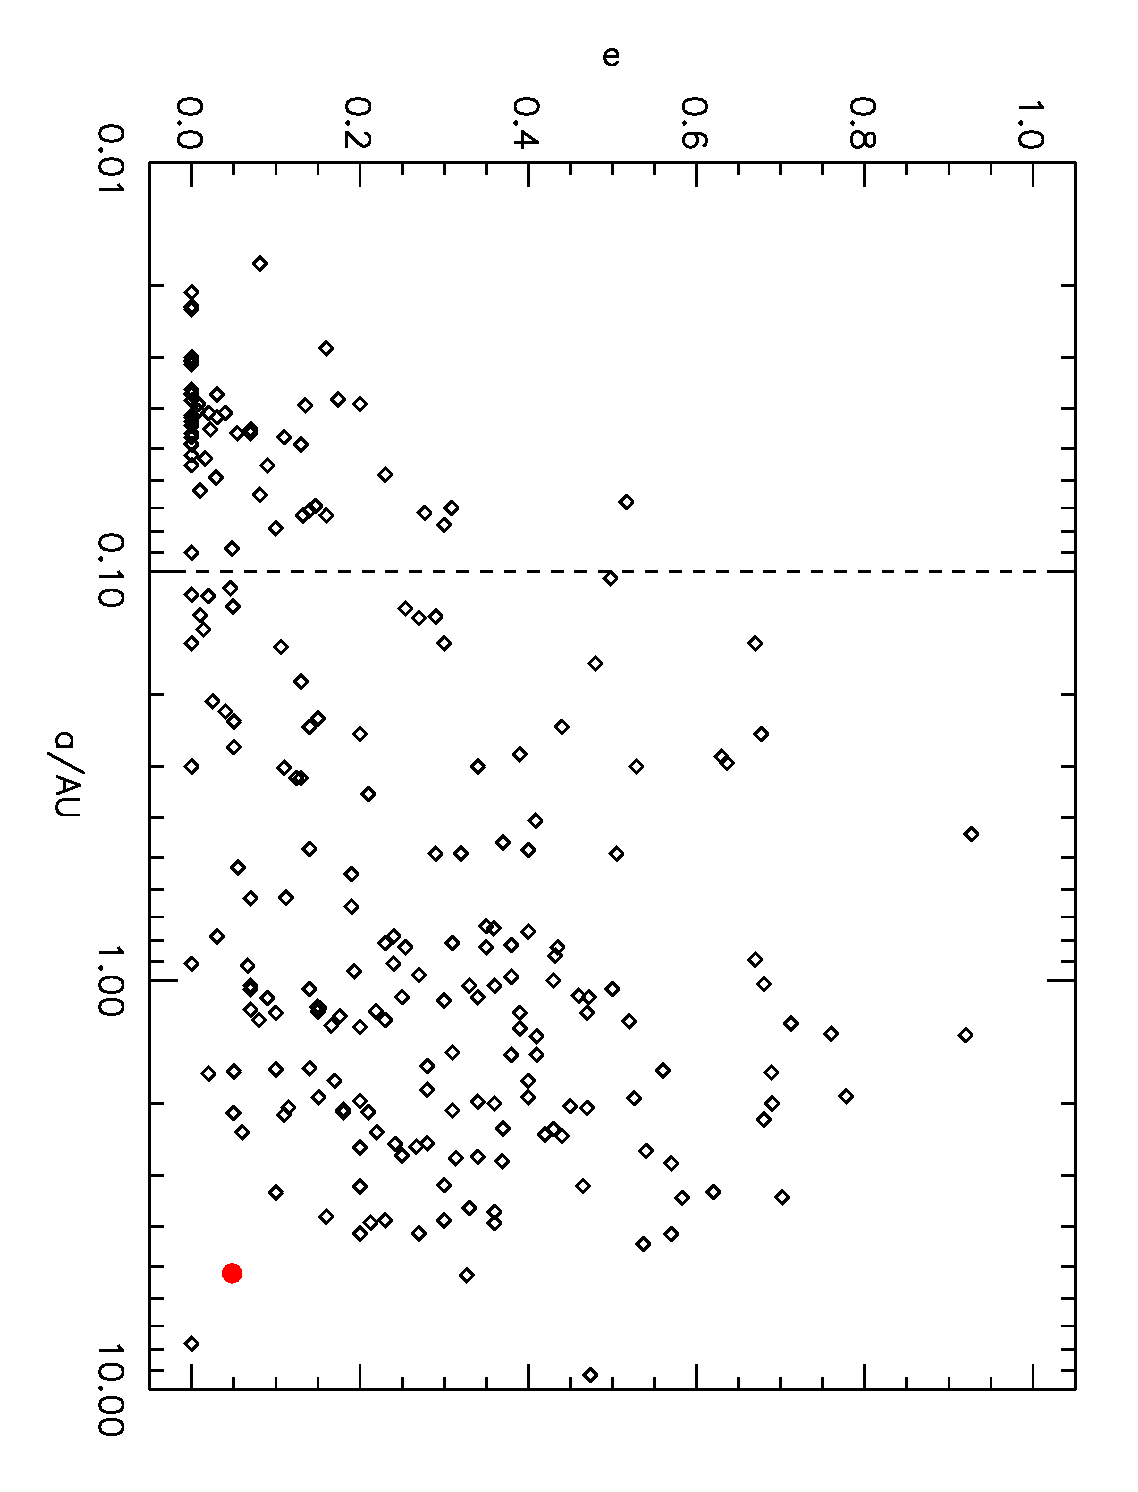
\includegraphics[angle=90,width=.90\textwidth]{1_rvplanetseccs}
\caption[Orbital eccentricity distribution of known exoplanets]{%
Orbital eccentricities of known exoplanets as a function of their orbital distance.
Jupiter is shown for comparison as a {\it red, filled circle}.
Most of the hot Jupiters (those to the left of the {\it dotted line}) have negligible eccentricity as expected from tidal circularization.%
}
\label{cha:intro:sec:methods:sub:rv:fig:rve}
\end{center}
\end{figure}

Many of the known extrasolar gas giants have orbital periods much less than that of Jupiter (again, see figure~\ref{cha:intro:sec:methods:sub:rv:fig:rv}), much to the surprise of the early discoverers.
Extrasolar gas giants that orbit their stars within 0.1\,AU are known as {\it hot Jupiters}, referring to the intense insolation experienced in a relative orbit well inside that of Mercury.
Tidal interactions (\citealp[see, e.g.,][]{Rasio_Ford:Science:1996a}) with the nearby star result in circular orbits for most of these close-in planets (see figure~\ref{cha:intro:sec:methods:sub:rv:fig:rve}).
Several planet searches such as this thesis work concentrate on these objects as they are both easier to find (due to their rapidly repeating signals) and fascinating to study (due to their extreme environment close to the star).
The proximity to the star also increases the probability that they will be observed to pass across the stellar disk.
The radial-velocity method achieves its full potential when combined with such transit observations, as this combined method allows a precise estimate of the mass and radius of the planet.

\subsection{Transits}
\label{cha:intro:sec:methods:sub:trans}

For every system of gravitationally bound celestial objects, there is a probability that we will observe these objects passing in front of each other, eclipsing the light from the other.
In the case of a hot Jupiter with a radius $\rp$ in a circular orbit around a star of radius \rstar, this probability is given by:
\begin{eqnarray*}
P & = & \frac{\rp + \rstar}{a},\\
 & \simeq & \frac{\rstar}{a},\\
  & \simeq & 10\% \left( \frac{\rstar}{\rsun} \right) \left( \frac{a}{0.05 AU} \right)^{-1},
\end{eqnarray*}
where 0.05\,AU is the median orbital distance for systems containing hot Jupiters \citep{Sackett:POSS:1999a}.
A planet in an 0.05\,AU orbit around a solar-sized star (with $P\sim10$\%) is therefore an ideal candidate to monitor for the transit of the planet across the star.

The passage of the planet across the stellar disk will block light from the star and reduce the flux by $\Delta F$.
For example, a transit of the Sun by Jupiter would block $\sim$1\% of the sunlight.
Assuming that \rstar\ can be determined from spectroscopy, the radius of the planet can then be calculated from:
\begin{eqnarray*}
r_{p} & = & {\rstar} \sqrt{\Delta F}.
\end{eqnarray*}
Such a transit would have a duration $D$ of :
\begin{eqnarray*}
D = \frac{P}{\pi} \arcsin{\left( \frac{\rstar}{a \sin{i}}
\sqrt{\left(1+\frac{\rp}{\rstar}\right)^2 - b^2} \right)},
\end{eqnarray*}
where $b$ $(=a\cos{i}/\rstar)$ is the impact parameter \citep{Seager_Mallen-Ornelas:apj:2003a}.
For a Jupiter-sized planet that transits the equator of a solar-type star with a 4-day period, the transit duration $D\sim2.5$\,hours.

\begin{figure}
\begin{center}
\centering
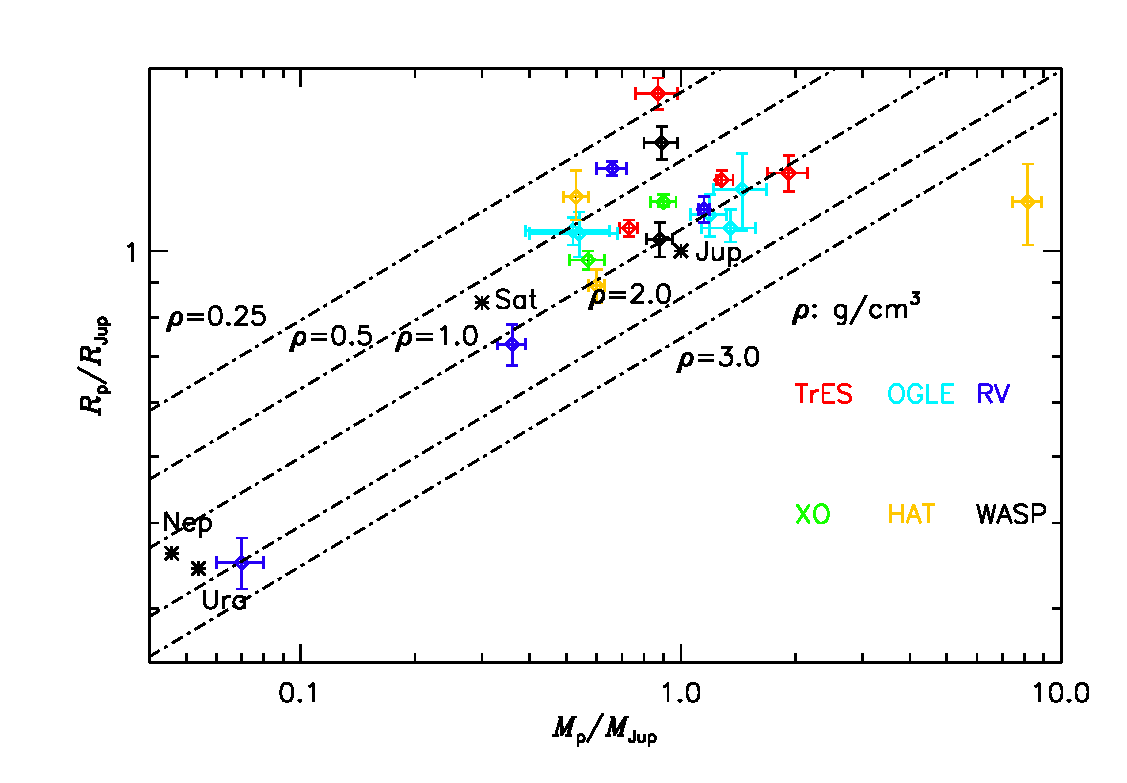
\includegraphics[width=.90\textwidth]{1_radii}\\
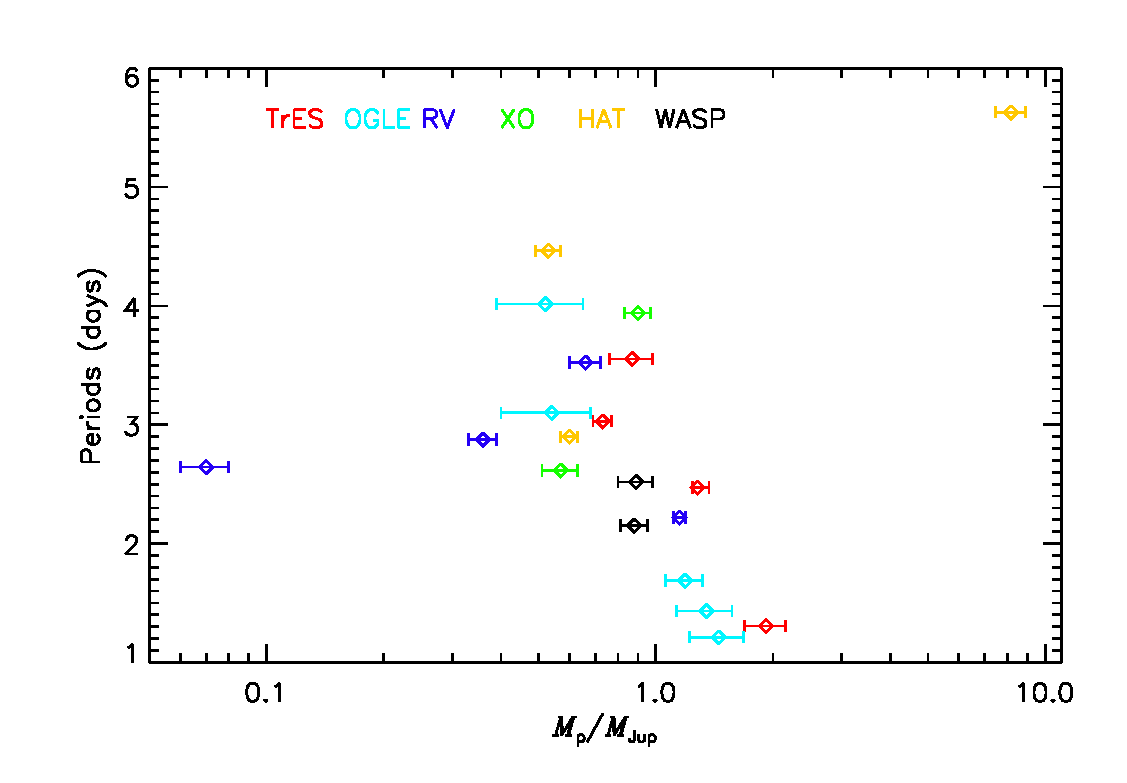
\includegraphics[width=.90\textwidth]{1_periods}\\
\caption[Mass-radius and mass-period relations for transiting planets]{%
Mass-radius ({\it top}) and mass-period ({\it bottom}) relations for the transiting planets known at the time of writing.
The {\it dot-dashed lines} represent different densities.
There is a spread of radii for planets of the same mass, and reproducing the largest radii is still beyond current structural models.
There also appears to be a decreasing trend in mass with period in the {\it bottom panel}.
In the $\sim$1--2-day period range, the planets all have $\mp \geq \mjup$.
This may indicate different formation mechanisms for these planetary systems than those at longer periods.
}
\label{cha:intro:sec:methods:sub:trans:fig:tp}
\end{center}
\end{figure}

In order for a transit to occur, the orbital inclination must be close to $90\degr$, hence the minimum mass derived for a transiting planet using equation~\ref{cha:intro:sec:methods:sub:rv:eqn:mpsini} is a close approximation of the true planetary mass.
By combining observations of transits and radial-velocity variations, astronomers have obtained mass and radius precise estimates of 20 transiting exoplanets (at the time of writing; see figure~\ref{cha:intro:sec:methods:sub:trans:fig:tp}) with which to test structural models for these giant balls of gas.
(For reference, I have placed tables of the properties of these transiting systems in appendix~\ref{cha:prop}.)
The masses of the transiting planets are clustered around $1\,\mjup$.
However, the discovery of the least massive (\gjFTSb) and most massive (\hatptwob) transiting planets to date suggest that over time the mass distribution will resemble more that of the radial-velocity planets (see figure~\ref{cha:intro:sec:methods:sub:rv:fig:rv}).

Figure~\ref{cha:intro:sec:methods:sub:trans:fig:tp} also shows the variation in orbital period with mass.
Although results thus far are limited by small number statistics, it appears that the more massive transiting planets have shorter orbital periods, and every $\mp<1\,\mjup$ planet has an orbital period greater than 2\,days.
This trend, which is in the opposite direction to the corresponding trend for the known radial-velocity planets (see figure~\ref{cha:intro:sec:methods:sub:rv:fig:rv}), was first noted by \citet*{Mazeh_Zucker_Pont:mnras:2005a} and \citet*{Gaudi_Seager_Mallen-Ornelas:apj:2005a}.
If the trend continues to be observed as more transiting planets are discovered in the range of orbital periods 1--5\,days, it may indicate a different origin for the planets with $\sim$one-day periods, perhaps by tidal capture rather than inward migration \citep{Gaudi_Winn:apj:2007a}.

In contrast to the number of known eccentric radial-velocity planets at small orbital separations (see figure~\ref{cha:intro:sec:methods:sub:rv:fig:rve}), there are only two known transiting planets (\gjFTSb\ and \hatptwob) in this category.
Again, over time when more transiting systems are known, it is likely that this number will significantly increase.

As well as providing the most precise masses and radii known for extrasolar planets, nearby transiting planets present some other unique opportunities to study their nature:
\begin{enumerate}
\item
Space-based telescopes offer the promise of exquisitely precise transit light curve with which to look for evidence of rings and satellites orbiting the gas giant \citep[see, e.g.,][]{Brown_Charbonneau_Gilliland:apj:2001a}.
\item
Radial-velocity observations of the star during transit can measure the strength of the Rossiter-McLaughlin effect \citep{McLaughlin:apj:1924a,Rossiter:apj:1924a}, an apparent radial-velocity variation caused by the blocking of light from the differentially rotating star.
The strength of the variation indicates the misalignment of the orbital and rotation axes of the system.
\item
We can also observe the starlight as it transmits through the planetary atmosphere during transit, and look for spectral features indicative of the chemical composition of the planet~\citep{Charbonneau_Brown_Noyes:apj:2002a, Vidal-Madjar_Lecavelier-des-Etangs_Desert:nat:2003a, Vidal-Madjar_Desert_Lecavelier-des-Etangs:apjl:2004a, Deming_Brown_Charbonneau:apj:2005a, Barman:apjl:2007a}.
\item
The relative flux of a hot Jupiter to that of the star is greatest in the infrared.
Since a transiting system undergoes a secondary eclipse as well as a primary eclipse (the transit), we can estimate the strength of this emission by comparing the system flux before the secondary eclipse, and the flux during the secondary eclipse when the star blocks the planetary flux.
Infrared emission has already been observed from several transiting planets using \spi\ \citep[see, e.g.,][]{Charbonneau_Allen_Megeath:apj:2005a, Deming_Seager_Richardson:nat:2005a}, and recently the first spectra of exoplanets were obtained \citep{Richardson_Deming_Horning:Nature:2007a, Swain_Bouwman_Akeson:preprint:2007a, Grillmair_Charbonneau_Burrows:apjl:2007a}, as well as the first map of the emission variation across a planet \citep{Knutson_Charbonneau_Allen:nat:2007a}.
\end{enumerate}

\section[Formation, Structure, and Composition of Highly-Irradiated Gas Giants]
{Formation, Structure, and Composition of \\ Highly-Irradiated Gas Giants}
\label{cha:intro:sec:form}

Transiting systems provide precise measurements of planetary masses and radii and facilitate the direct study of the orbital alignment and spectral features of the planet.
In this section, I will explain how these observations serve as important constraints for models of the initial formation, internal structure and atmospheric composition of these distant gas giants.
Before the discovery of these giants in such extreme environments, the only constraints of theoretical models were the solar system gas giants.
Models based on our own planetary system proved to be inadequate for hot Jupiters.

\subsection{The Birth of Giants}
\label{cha:intro:sec:form:subsec:birth}

The canonical model for the formation of gas giants prior to the discovery of hot Jupiters nicely reproduced the giant planets of our solar system.
In this core accretion model \citep[see, e.g.,][]{Pollack:araa:1984a,Pollack_Hubickyj_Bodenheimer:icarus:1996a}, the gas giant begins as a protoplanetary core within a nebular disk and grows through collisions with other protoplanets and the accretion of gas from the surrounding disk.
When the core is massive enough, a period of runaway gas accretion occurs, and a giant planet is born.
This core formation relies on a suitable quantity of icy particles in the surroundings to form planetesimals.
With the discovery of \mbox{51\,Peg\,b} \citep{Mayor_Queloz:nat:1995a}, a giant planet close to its star and well inside the {\it ice line} (the boundary beyond where most material is in solid, rather than gaseous, form), the validity of this theory was called into question: how could this planet have formed a solid core so close to the star?

The most likely explanation is that hot Jupiters like \mbox{51\,Peg\,b} formed outside the ice line (as did the solar system gas giants), and then moved or {\it migrated} inward toward the star (\citealp{Goldreich_Tremaine:apj:1980a}; Lin, Bodenheimer, \& Richardson~\citeyear{Lin_Bodenheimer_Richardson:nat:1996a}; \citealp{Trilling_Benz_Guillot:apj:1998a}).
This migration is enabled by gravitational interactions between the planet and the disk.
Whether the migration is halted by some mechanism or the observed planet survived simply because the disk dissipated in time to prevent further migration is still unresolved.

\subsection{A Core or Not a Core, That is the Question}
\label{cha:intro:sec:form:subsec:core}

An alternative formation model for gas giants was proposed by~\citet{Boss:sc:1997a}.
In his gravitational instability model, gas giants can be formed rapidly as collapsing instabilities in the nebula.
A consequence of this rapid formation is that the gas giant is thought not to have a substantial core, although some heavy elements may be accumulated through planetesimal bombardment.

The ability to measure the masses and radii of hot Jupiters allows us to test for the presence or absence of cores, and thus differentiate between the two models.
Models of gas giants that include a substantial core have a smaller radius for the planet, and this effect is larger for the less massive giants.
There is some evidence for core accretion in the observations of transiting planets.
\hdOFNb\ is a transiting hot Saturn whose radius is so small for its mass that a large core of approximately 70\,\mearth\ of heavy elements is implied by the models~\citep{Sato_Fischer_Henry:apj:2005a, Charbonneau_Winn_Latham:apj:2006a, Fortney_Saumon_Marley:apj:2006a}.

However, ever since the discovery of \hdTZNb, we have struggled to adapt these models to explain every extrasolar mass-radius relation.
We have now identified several transiting gas giants whose radii exceed our predictions for their masses;
the values for the remaining planets are in agreement with models either with or without a core \citep[see,][for a review]{Laughlin_Wolf_Vanmunster:apj:2005a, Charbonneau_Brown_Burrows:PPV:2007a}.

In order to explain these ``inflated'' planets, several additional energy sources were proposed that could slow the contraction of the planet after formation, and would result in a larger radius.
\citet*{Bodenheimer_Lin_Mardling:apj:2001a} and \citet*{Bodenheimer_Laughlin_Lin:apj:2003a} suggested the presence of an additional but unseen planet in the transiting system that would continuously pump the orbital eccentricity of the detected planet.
The tidal circularization of this nonzero eccentricity would produce the energy internal to the planet required to maintain the large radius.
\citet{Winn_Holman:apjl:2005a} proposed a similar tidal dissipation, this time of a nonzero obliquity of a planet in a Cassini state.
The explanation put forth by \citet{Guillot_Showman:aa:2002a} and \citet{Showman_Guillot:aa:2002a} was that some of the intense insolation creates atmospheric winds and thereby contributes thermal energy to the interior.
\citet{Burrows_Hubeny_Budaj:apj:2007a} explored the effect of substantially increased planetary metallicity on the opacity of the planetary atmosphere and suggested that the resultant increased opacity would act to slow the heat loss from and hence contraction of the planet.
\citet*{Burrows_Sudarsky_Hubbard:apj:2003a} and \citet{Baraffe_Chabrier_Barman:aa:2003a} pointed out an effect due to the difference between the observed planetary radius (corresponding to an optical depth of unity at some wavelength) and the theoretical radius (at the 1-bar level) that could account for 5\% of the discrepancy between the two.

However, no satisfying solution has been found to date.
The kinetic energy source of \citet{Guillot_Showman:aa:2002a} should apply to every hot Jupiter, yet \hdTZNb\ and \tresOne\ have similar masses but significantly different radii.
\citet{Deming_Seager_Richardson:nat:2005a} refuted the possibility that tidal damping of a nonzero eccentricity was an energy source for the inflated planet \hdTZNb\ by deriving a negligible eccentricity from observations of a secondary eclipse.
Also, \citet*{Fabrycky_Johnson_Goodman:apj:2007a} has rejected obliquity tides as not providing enough energy through dissipation to account for large radii of hot Jupiters.

\subsection{Extrasolar Atmospheres}
\label{cha:intro:sec:form:subsec:atm}

Although giant planets consist mainly of gas, namely molecular hydrogen and helium, both the absorption rate of incident radiation, and the emission from (and hence cooling rate of) the planet is determined mostly by a thin outer layer of these gaseous molecules.
This thin layer is called the {\it atmosphere} of the planet.
The composition of the atmosphere, and the gas giant itself, is expected to be roughly the composition of the nebula from which it formed, although substantially enriched due to bombardment of planetesimals.
The presence or absence of specific chemical species in the atmosphere is then dependent on the temperature and pressure gradients of the planet.
The metallicity of the atmosphere can be a significant effect.
The infrared color of \tresOne~\citep{Charbonneau_Allen_Megeath:apj:2005a} is too red when compared to model spectra and other planets, and \citet{Fortney_Marley_Lodders:apjl:2005a} explained this as due to a metallicity 3--5 times solar.

Once again, the extreme nature of the environment of hot Jupiters presents a new challenge to models of gas giants, this time of their atmospheres.
Jupiter has an effective temperature of 125\,K, has an intrinsic luminosity due to ongoing contraction roughly equal to its luminosity due to reradiated solar flux, and almost completely redistributes the thermal energy from this flux from the dayside to the night-side of the planet.
In contrast, hot Jupiters have equilibrium temperatures of up to 1500\,K.
Of their luminosity, 99.99\% is due to the re-radiation of the insolation \citep{Marley_Fortney_Seager:PPV:2007a}.
This intense radiation may result in hot substellar spots, and could cause day-night temperature differences of up to $\sim$500\,K, and winds of up to 2\,\kms~\citep{Showman_Guillot:aa:2002a}.
The efficiency of the redistribution of the heat from this spot may vary from planet to planet.

Due to the high effective temperatures, atmospheric models predict different dominant molecular absorbers in the spectra of the hot Jupiters than of the solar system giants.
At the visible wavelengths, Na and K produce strong absorption features, whereas in the infrared, H$_2$O, CO, CH$_4$, and CH$_3$ are all noticeable absorbers.
The exact planetary spectrum depends on the amount of insolation absorbed by the planet, the redistribution of the resultant thermal energy, and the presence or absence of high clouds of condensates.
Unlike the solar system giants for which we have direct estimates of the solar flux and of the chemical compositions, we can be certain only of the incident radiation onto these planets.
However, if we measure the amount of flux from the night-side of a transiting planet (during a transit) and from the day-side (during a secondary eclipse), we can deduce how much energy is being transported from the dayside, and hence measure the efficiency of this redistribution.

Understanding the atmospheric makeup of the hot Jupiters may provide us with an explanation for the inflated exoplanets, as the predictions for these radii are dependent on understanding the cooling rates of the planets.


\section{Thesis Motivation---Past and Present}
\label{cha:intro:sec:motivation}

At the beginning of my thesis work, only one transiting planet, \hdTZNb, was known.
The radius of this planet was larger than could be explained by extrapolating models of solar system gas giants to account for intense insolation.
This made the discovery of additional transiting planets very important to allow determination of whether this planet was merely an anomaly.
Transit surveys also held the promise of being the most effective way to obtain precise planetary masses and radii to provide constraints for models.
In contrast to the radial-velocity surveys of individual stars, transit surveys monitor thousands of stars at a time for evidence of a planetary companion, although the expected frequency of detections was not well understood.
With the TrES team's discovery of \tresOne~\citep{Alonso_Brown_Torres:apjl:2004a}, wide-field surveys proved our ability to find transiting planets around stars bright enough to provide these desired precise constraints.
It was clear that my wide-field transit survey could make a substantial contribution even by discovering only one or two transiting planets.
By extending the coverage of the parameter space for exoplanets, I could hope to improve the understanding of the wide range of radii for planets of similar masses.
The bright stars that I would find as part of my survey would also be ideal targets for detailed studies of the atmosphere and neighboring objects with space-based telescopes.

The goals that motivate my thesis work still hold today, since the number of known transiting planets (19) is still quite low.
The planets found by TrES and other surveys continue to be much sought after, and quickly observed with the best instruments available to uncover the true nature of each planet.

\section{Thesis Outline}
\label{cha:intro:sec:outline}

The goals of my thesis were to both detect and explore new transiting planets.
Much of my thesis work involved participation in the Trans-atlantic Exoplanet Survey (TrES), a network of three ten-centimeter optical telescopes used to search for nearby transiting planets.

For four years, I have operated and maintained the telescope Sleuth at Palomar Observatory, obtaining observations of TrES fields almost every night (weather permitting).
I have reduced these observations, and searched the resulting time series of field stars for transit signals.
For each transit candidate that I identified, it has been my responsibility to then coordinate follow-up spectroscopic observations, obtained by D.~Latham and collaborators, and follow-up photometric observations, obtained by me and several TrES collaborators.
I pursued my own follow-up photometry using Sherlock \citep{Kotredes_Charbonneau_Looper:2004a} or the Palomar 1.5-meter telescope \citep[see, e.g.,][for an example of the 1.5-meter photometry]{Holman_Winn_Latham:apj:2006a}, and performed modeling of this photometry to derive precise transit parameters.
Based on the results of each new set of observations, I removed false positives from my candidate list.

Twice during my thesis, I obtained high-dispersion observations of my most promising transit candidates with Keck/HIRES, aided by D.~Charbonneau, G.~Torres, and A.~Sozzetti, who performed the rapid data analysis needed to review the data while still at Keck.
The subsequent required blend analysis and photometric modeling of the three planets that I discovered were performed by G.~Torres and D.~Charbonneau, respectively.

Having discovered \tresTwo, I then turned my attention to analyzing the \spi\ observations of this planet, obtained by my collaborator J.~Harrington.
The theoretical interpretation of the data was carried out in collaboration with S.~Seager.

Most of the chapters in this thesis are based on material published during my time at Caltech.
I have presented them in a logical order, rather than ordered by publication date.

In chapter~\ref{cha:and0}, I outline how I obtained observations of 26,495 stars in a single field using Sleuth, and my analysis of the data.
I present six candidates that I identified from a transit search of the photometry.
I explore the methods used by the TrES team to reject astrophysical false positives, and explain how the six stars were culled from our candidate transiting system list.
In this chapter, I also demonstrate the advantages of a multisite network such as TrES for obtaining better phase coverage and confirming the reliability of these candidates.

Most transit surveys have obtained significant experience with these typical astrophysical false positives.
In chapter~\ref{cha:gsc}, I discuss an early example of a more insidious false positive, \gscOTE, that I identified as a candidate transiting planet.
This system proved to be a solitary star blended with an eclipsing binary.
The relative faintness of the binary prevented the detection of its radial-velocity signal.
Multicolor photometry revealed a color-dependent eclipse, indicative of the binary nature.
In this chapter, I go into more detail about how I produce light curves from Sleuth photometry and select transit candidates.

In chapter~\ref{cha:tres2}, I present the discovery in one of the Sleuth fields of a massive gas giant \tresTwo\ that was confirmed from the spectroscopic orbit derived from my observations with Keck/HIRES.
\tresTwo\ is the first transiting planet known to reside in the field of view of the upcoming NASA {\it Kepler} mission that will search for new exoplanets.
Similarly, in chapter~\ref{cha:tres3}, I present \tresThree, another massive transiting planet from a Sleuth field, this time with a very-short orbital period.
This discovery has further cemented the hypothesis that the nearby exoplanets discovered by wide-field transit surveys and the more distant gas giants found by narrow-field transit surveys have the same intrinsic period distribution.
I have also included in appendix~\ref{cha:tres4} the discovery paper for \tresFour, the third planet found in a Sleuth field.
This planet has the largest radius and lowest density of the currently known transiting planets.

Although each newly discovered transiting planet automatically provides a new constraint for theoretical structural models for these Jovian planets, the nearby transiting planets also present promises of a more detailed exploration.
{\it Spitzer} has been a leading source of new information about exoplanets, and in chapter~\ref{cha:spitzer}, I present my analysis of the first \spi/IRAC observations of \tresTwo, and determine a negligible orbital eccentricity for this hot Jupiter. There is no evidence of strong atmospheric absorption from these observations, but future analysis including additional \spi\ observations will be more conclusive.

Finally, I examine the yield of planets from this survey in comparison with predictions.
In chapter~\ref{cha:human}, I present initial results from a study of my ability to recover fake transit light curves injected into real data from a TrES field.
Rather than just concentrate on the recovery rate of the transit-search algorithm I employ, I explore the human element of identifying worthy planet candidates, and the resultant recovery rate of transit candidates.

The photometric data from Sleuth have also been of value in the study of eclipsing binaries. As this is not related to my thesis goals, I simply refer the reader to \citet{Creevey_Benedict_Brown:apjl:2005a} and Devor et al.~(2007, in preparation) as examples of this use of Sleuth data.
